\section{Project introduction}
\label{project_introduction}
% 1/3 rapporter har noe tekst her. Enn så lenge så prioriterer vi ikke det.


\subsection{Project goal}
The goal of this project is to develop software for a customer and document the process of the development. The group was issued the task of researching and developing an application aimed at the medical industry. This was to be a proof-of-concept application to shed light upon all the various aspects one has to consider while developing for the health sector. With a presumed, future smart device, running on the Android platform, the customer wanted an application that was able to connect wirelessly to existing hospital information systems in order to store ultrasound images and related data. This device is capable of receiving ultrasound images and video from a connected ultrasound probe over a common wired interface. The application would then be able to download relevant information about a patient, combine it with examination data (images and meta) and upload it to existing hospital information systems. Being an international company, the customer want this to work with different existing hospital information systems on an international scale.

\subsection{Customer}
The customer is the international consulting firm Capgemini. They are collaborating with GE Healthcare, a company providing medical technologies and services around the world \cite{gehealthcare}. GE Vingmed Ultrasound is a division of GE Healthcare based in Horten, Norway. They are the team behind the handheld ultrasound device Vscan (Figure \ref{vscandevice}). Vscan is an award-winning \cite{vscan_awards} portable ultrasound device used by doctors worldwide. GE Vingmed is looking to expand the functionality of this device, and this is the basis for the project.

\begin{figure}[H]
\centering
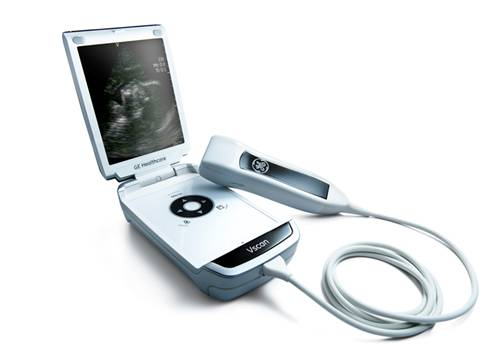
\includegraphics[scale=0.60]{img/vscan.jpg}
\caption{The Vscan Device}
\label{vscandevice}
\end{figure}

\subsection{Project scope}
The original intention of the customer was for us to deliver a system that worked on a global scale, meeting legal requirements in hundreds of countries, working across several different standards and protocols for exchanging medical information and communicating with several different existing hospital information systems. It did not take a lot of research to realize that this was a more than an ambitious goal \cite{metricFuckton}. Therefore, an agreement with the customer was made to reduce the scope of the project. Not even the Norwegian hospitals in the same region have agreed on a standard IT infrastructure, so we decided to focus on the largest institution in Norway, Oslo University Hospital (OUS), and the systems in use there.

This means researching and learning how the largest vendors of \emph{Patient Administration Systems} (PAS) and \emph{Electronic Medical Records} (EMR) work. Along with this we will look at future standards and solutions.

\subsection{Project constraints and resources}
Some of the constraints for this project are the limited documentation regarding software implementation of the EMRs and the systems that surrounds them, as well as the use of proprietary technology by many of the EMRs. This have made it hard for the group as developers to design and implement the functionality for communication with these systems, as well as testing the application against the systems it is designed for. 

To counter this issue, we have actively been trying to get in touch with people in the industry that might be able to help with understanding the necessary communication between the EMR clients and servers.